% 6-10 pages, 9pt font
%
% Topics:
%
% * Machine learning based autotuning.
% * Representative benchmarking.
% * Automatic fault tolerance.
% * Run-time adaption.
%

% The following \documentclass options may be useful:
%
% preprint      Remove this option only once the paper is in final form.
% 10pt          To set in 10-point type instead of 9-point.
% 11pt          To set in 11-point type instead of 9-point.
% authoryear    To obtain author/year citation style instead of numeric.
\documentclass[nonatbib,preprint,nocopyrightspace,9pt]{sigplanconf}

%%%%%%%%%%%%%%%%%%%%%%%%%
%% Document and Layout %%
%%%%%%%%%%%%%%%%%%%%%%%%%

% Fix for multiple "No room for a new \dimen" errors.
%
% See: http://tex.stackexchange.com/questions/38607/no-room-for-a-new-dimen
%
\usepackage{etex}

\usepackage[utf8]{inputenc}

% Fix for "'babel/polyglossia' detected but 'csquotes' missing"
% warning. NOTE: Include after inputenc.
%
\usepackage{csquotes}

% Make internal macro definitions accessible,
% e.g. \@title, \@date \@author.
\makeatletter

% Multi-column support.
\usepackage{multicol}

% A useful package which includes macros like \ifdef{}{}{}:
%
\usepackage{etoolbox}

% Uncomment the following line to remove column separation:
%
%\setlength{\columnsep}{5mm}

% Allow user-defined warning and error filters.
%
\usepackage{silence}


%%%%%%%%%%%%%%%%%%%%%
% Table of Contents %
%%%%%%%%%%%%%%%%%%%%%

% % Set chapter and section numbering depth:
% %
% \setcounter{secnumdepth}{2}


%%%%%%%%%%%%%%%%
% Bibliography %
%%%%%%%%%%%%%%%%
\usepackage[%
    backend=biber,
    style=numeric-comp,
    % style=numeric-comp,  % numerical-compressed
    sorting=none,        % nty,nyt,nyvt,anyt,anyvt,ynt,ydnt,none
    sortcites=true,      % sort \cite{b a d c}: true,false
    block=none,          % space between blocks: none,space,par,nbpar,ragged
    indexing=false,      % indexing options: true,false,cite,bib
    citereset=none,      % don't reset cites
    isbn=false,          % print ISBN?
    url=true,            % print URL?
    doi=false,           % print DOI?
    natbib=true,         % natbib compatability
  ]{biblatex}

% % Filter annoying and unavoidable biblatex warning:
\WarningFilter{biblatex}{Patching footnotes failed}

% Reduce the font size of the bibliography:
% \renewcommand{\bibfont}{\normalfont\scriptsize}

% Determine which BibTeX file to use:
%
% If available, use my Mendeley BibTex library, located in the home
% directory. Note that this is a relative path and will break if
% either this file or the BibTex library are moved. If the library is
% not present, use the local refs.bib file.
\newcommand{\BibResourceGlobal}{../../library.bib}
\newcommand{\BibResourceLocal}{refs.bib}

\IfFileExists{\BibResourceGlobal}
  {\newcommand{\BibResource}{\BibResourceGlobal}}
  {\newcommand{\BibResource}{\BibResourceLocal}}

\addbibresource{\BibResource}


%%%%%%%%%%%%%%
% Appendices %
%%%%%%%%%%%%%%

% Appendix package. Documentation:
%
%  http://mirror.ox.ac.uk/sites/ctan.org/macros/latex/contrib/appendix/appendix.pdf
%
% Package options:
%
% toc      - Put a header (e.g., `Appendices') into the Table of Contents
%            (the ToC) before listing the appendices. (This is done by
%            calling the \addappheadtotoc command.)
% page     - Puts a title (e.g., `Appendices') into the document at the
%            point where the appendices environment is begun. (This is
%            done by calling the \appendixpage command.)
% title    - Adds a name (e.g., `Appendix') before each appendix title in
%            the body of the document. The name is given by the value
%            of \appendixname. Note that this is the default behaviour
%            for classes that have chapters.
% titletoc - Adds a name (e.g., `Appendix') before each appendix listed
%            in the ToC. The name is given by the value
%            of \appendixname.
% header   - Adds a name (e.g., `Appendix') before each appendix in page
%            headers.  The name is given by the value
%            of \appendixname. Note that this is the default behaviour
%            for classes that have chapters.
\usepackage[title, titletoc]{appendix}


%%%%%%%%%%%%%%%%%%%%%%%%%%%%%%%%%%%%%
%% Figures, footnotes and listings %%
%%%%%%%%%%%%%%%%%%%%%%%%%%%%%%%%%%%%%

%\usepackage{float}
%\restylefloat{figure}

% Use bold ``(Figure|Table|Listing)'' caption text.
%\usepackage[margin=1cm]{caption}

% Set the font for captions.
% \renewcommand{\captionfont}{\small}
% Set the font for caption labels.
% \renewcommand{\captionlabelfont}{\footnotesize\bf}

% Use arabic numbers for footnote.
%\renewcommand{\thefootnote}{\arabic{footnote}}

% Ensure that footnotes always appear at the bottom of pages.
%\usepackage[bottom]{footmisc}

% Reset the footnote counter on every page.
%\usepackage{perpage}
%\MakePerPage{footnote}

% Pre-requisites for rendering upquotes in listings package.
\usepackage[T1]{fontenc}
\usepackage{lmodern}
\usepackage{textcomp}

% Pseudo-code listings.
\usepackage{algorithm}
\usepackage{algpseudocode}
\newcommand{\Break}{\State \textbf{break} }
\algblockdefx[Loop]{Loop}{EndLoop}[1][]{\textbf{Loop} #1}{\textbf{End
    Loop}}

\algrenewcommand\ALG@beginalgorithmic{\footnotesize}

% Code listings.
\usepackage{listings}

% Set \ttfamily to use courier fonts.
%
% See: http://tex.stackexchange.com/a/33686
%
\usepackage{courier}

\lstset{frame=bt,                    % Add top and bottom frame lines
        breaklines=true,             % Force line wrapping
        captionpos=b,                % Place caption below listing
        numbers=left,                % Add left-side line numbers
        basicstyle=\scriptsize\ttfamily, % Set font size and type
        showstringspaces=false,      % Don't show visible whitespace
        numberstyle=\tiny,
        upquote=true,                % Use upright quotes, not curly
        commentstyle=\bfseries}      % Embolden comments

% Use (*@ @*) to escape LaTeX commands within listings.
\lstset{escapeinside={(*@}{@*)}}

% Add 10pt space between chapters in TOC listings entries:
%\let\Chapter\chapter
%\def\chapter{\addtocontents{lol}{\protect\addvspace{10pt}}\Chapter}


%%%%%%%%%%%%%%%%%%%%%%%%
%% Graphics and maths %%
%%%%%%%%%%%%%%%%%%%%%%%%
\usepackage{amsmath}

% Vector notation, e.g. \vv{x}:
%
\usepackage{esvect}

% Additional amsmath symbols, see:
%
% http://texblog.org/2007/08/27/number-sets-prime-natural-integer-rational-real-and-complex-in-latex/
%
\usepackage{amsfonts}
\usepackage{amssymb}

\usepackage{graphicx}
\usepackage{mathtools}
\usepackage{tikz}
\usepackage{tikz-qtree}

% Provide bold font face in maths.
\usepackage{bm}

\usepackage{subcaption}
\expandafter\def\csname ver@subfig.sty\endcsname{}

% Define an 'myalignat' command which behave as 'alignat' without the
% vertical top and bottom padding. See:
%     http://www.latex-community.org/forum/viewtopic.php?f=5&t=1890
\newenvironment{myalignat}[1]{%
  \setlength{\abovedisplayskip}{-.7\baselineskip}%
  \setlength{\abovedisplayshortskip}{\abovedisplayskip}%
  \start@align\z@\st@rredtrue#1
}%
{\endalign}

% Define additional operators:
\DeclareMathOperator*{\argmin}{arg\,min}
\DeclareMathOperator*{\argmax}{arg\,max}

\DeclareMathOperator*{\gain}{Gain}

% Skeleton operators.
\DeclareMathOperator*{\map}{Map}
\DeclareMathOperator*{\reduce}{Reduce}
\DeclareMathOperator*{\scan}{Scan}
\DeclareMathOperator*{\stencil}{Stencil}
\DeclareMathOperator*{\zip}{Zip}
\DeclareMathOperator*{\allpairs}{All\,Pairs}

% Maths plots using pgfplots, see:
%
%     http://pgfplots.sourceforge.net/pgfplots.pdf
%
\usepackage{pgfplots}

% Disable compatability mode.
%
\pgfplotsset{compat=1.12}

% Gantt charts using pgfgantt, see:
%
%     http://www.ctan.org/pkg/pgfgantt
%
\usepackage{pgfgantt}

% Fix milestone aspect ratio by defining a custom element.
\newganttchartelement*{mymilestone}{
  mymilestone/.style={
    shape=diamond,
    inner sep=2pt,
    draw=black,
    top color=black,
    bottom color=black,
  }
}

% Tikz flowchart configuration.
\usetikzlibrary{shapes,arrows,shadows,fit,backgrounds}
\tikzstyle{decision} = [diamond,
                        draw,
                        text width=4.5em,
                        text badly centered,
                        node distance=3cm,
                        inner sep=0pt]
\tikzstyle{block}    = [rectangle,
                        draw,
                        text width=5em,
                        text centered,
                        node distance=3cm,
                        minimum height=4em,
                        inner sep=.2cm]
\tikzstyle{line}     = [draw, -latex']

% Add dirtree picture style, see:
%
%     http://tex.stackexchange.com/a/34268
%
\newcount\dirtree@lvl
\newcount\dirtree@plvl
\newcount\dirtree@clvl
\def\dirtree@growth{%
  \ifnum\tikznumberofcurrentchild=1\relax
    \global\advance\dirtree@plvl by 1
    \expandafter\xdef\csname dirtree@p@\the\dirtree@plvl\endcsname{\the\dirtree@lvl}
  \fi
  \global\advance\dirtree@lvl by 1\relax
  \dirtree@clvl=\dirtree@lvl
  \advance\dirtree@clvl by -\csname dirtree@p@\the\dirtree@plvl\endcsname
  \pgf@xa=0.33cm\relax
  \pgf@ya=-\baselineskip\relax
  \pgf@ya=\dirtree@clvl\pgf@ya
  \pgftransformshift{\pgfqpoint{\the\pgf@xa}{\the\pgf@ya}}%
  \ifnum\tikznumberofcurrentchild=\tikznumberofchildren
    \global\advance\dirtree@plvl by -1
  \fi
}
\tikzset{
  dirtree/.style={
    growth function=\dirtree@growth,
    every node/.style={anchor=north},
    every child node/.style={anchor=west},
    edge from parent path={(\tikzparentnode\tikzparentanchor) |- (\tikzchildnode\tikzchildanchor)}
  }
}

% UML sequence diagram macros, see:
%
%     https://code.google.com/p/pgf-umlsd/
%
% Options:
%
%     underline - Underline object names
%
\usepackage[underline=false]{pgf-umlsd}

% Support for SVG graphics.
%
% NOTE that you must pass the "--shell-escape" argument to pdflatex to
% compile. NOTE also that images *MUST* be placed within the graphics
% path.
\usepackage{svg}
\graphicspath{{img/}}

%%%%%%%%%%%%%%%%%%%%%%
%% Tables and lists %%
%%%%%%%%%%%%%%%%%%%%%%

% Required to use labm8 exported tables.
%
\usepackage{booktabs}

% Required for full page-width tables.
\usepackage{tabularx}

%\usepackage{enumitem}
%\setenumerate{itemsep=0pt}

% Use no left margin for lists:
%\setlist{leftmargin=*}

\usepackage{longtable}

% Define column types L, C, R with known text justification and fixed
% widths:
\usepackage{array}
\newcolumntype{L}[1]{>{\raggedright\let\newline\\\arraybackslash\hspace{0pt}}m{#1}}
\newcolumntype{C}[1]{>{\centering\let\newline\\\arraybackslash\hspace{0pt}}m{#1}}
\newcolumntype{R}[1]{>{\raggedleft\let\newline\\\arraybackslash\hspace{0pt}}m{#1}}


%%%%%%%%%%%%%%%%%%%%%%%%%%%%%
%% Typesetting and symbols %%
%%%%%%%%%%%%%%%%%%%%%%%%%%%%%

% Adjustable font sizes in \Verbatim{}
\usepackage{fancyvrb}

%\usepackage{titlesec}
% Set section and paragraph heading fonts:
%\titleformat*{\section}{\Large\bfseries}
%\titleformat*{\subsection}{\normalsize\bfseries}
%\titleformat*{\subsubsection}{\normalsize}
%\titleformat*{\paragraph}{\large\bfseries}
%\titleformat*{\subparagraph}{\large\bfseries}

% Set section heading margins. Usage:
% \titlespacing*{<command>}{<left>}{<before>}{<after>}
%\titlespacing*{\section}{0pt}{.6em}{.3em}
%\titlespacing*{\subsection}{0pt}{.6em}{.2em}

% Set paragraph indentation size. Default is 15pt.
%\setlength{\parindent}{10pt}

% The line spacing can be globally set using \linespread:
%
% \linespread{1.2}

% Add a command \hr{} which will draw a horizontal rule the width of
% the text.
%
\newcommand{\hr}{\noindent\makebox[\linewidth]{\rule{\textwidth}{0.2pt}}}

% Add a command \br{} which will create a horizontal space of exactly
% one line height.
%
\newcommand{\br}{\hspace{\baselineskip}}

% Define a command to allow word breaking.
\newcommand*\wrapletters[1]{\wr@pletters#1\@nil}
\def\wr@pletters#1#2\@nil{#1\allowbreak\if&#2&\else\wr@pletters#2\@nil\fi}

% Define a command to create centred page titles.
\newcommand{\centredtitle}[1]{
  \begin{center}
    \large
    \vspace{0.9cm}
    \textbf{#1}
  \end{center}}

% Support hyperlinks using the \hyperref, \url and \href
% macros. Usage:
%
%    \hyperref[label_name]{''link text''}
%
%    \url{<my_url>}
%
%    \href{<my_url>}{<description>}
%
\usepackage{hyperref}

% Disable colored borders of links, cross-references etc in PDF output
\hypersetup{pdfborder={0 0 0}}

% Provide generic commands \degree, \celsius, \perthousand, \micro
% and \ohm which work both in text and maths mode.
\usepackage{gensymb}

%%%%%%%%%%%%%%%%%%%%%%%%%%%%%%%%%
%% Placeholder text generation %%
%%%%%%%%%%%%%%%%%%%%%%%%%%%%%%%%%

% Use either \blindtext or \libpsum to generate placeholder text. Also
% note the macros \blinditemize, \blindenumerate, \blinddescription.
\usepackage[english]{babel}
\usepackage{blindtext}
\usepackage{lipsum}


\begin{document}

\special{papersize=8.5in,11in}
\setlength{\pdfpageheight}{\paperheight}
\setlength{\pdfpagewidth}{\paperwidth}

\conferenceinfo{HLPGPGPU '16}{Month d--d, 20yy, City, ST, Country}
\copyrightyear{2016}
\copyrightdata{978-1-nnnn-nnnn-n/yy/mm}
\doi{nnnnnnn.nnnnnnn}

% Uncomment one of the following two, if you are not going for the
% traditional copyright transfer agreement.

%\exclusivelicense                % ACM gets exclusive license to publish,
                                  % you retain copyright

%\permissiontopublish             % ACM gets nonexclusive license to publish
                                  % (paid open-access papers,
                                  % short abstracts)

% \titlebanner{banner above paper title}        % These are ignored unless
% \preprintfooter{HLPGPGPU workshop '16}   % 'preprint' option specified.

% \title{Robust Autotuning of Stencil codes for GPUs with OmniTune}
% \title{Towards robust cross-architecture GPGPU patterns autotuning}
\title{Towards Collaborative Performance Tuning of Algorithmic Skeletons}

% \subtitle{Subtitle Text, if any}

\authorinfo{Chris Cummins\and Pavlos Petoumenos \and Michel Steuwer \and Hugh Leather}
           {University of Edinburgh}
           {c.cummins@ed.ac.uk, ppetoume@inf.ed.ac.uk, michel.steuwer@ed.ac.uk, hleather@inf.ed.ac.uk}

\maketitle

\begin{abstract}
  The physical limitations of microprocessor design have forced the
  industry towards increasingly heterogeneous designs to extract
  performance. This trend has not been matched with adequate software
  tools, leading to a growing disparity between the availability of
  parallelism and the ability for application developers to exploit
  it.

  Algorithmic skeletons simplify parallel programming by providing
  high-level, reusable patterns of computation. Achieving performant
  skeleton implementations is a difficult task; skeleton authors must
  attempt to anticipate and tune for a wide range of architectures and
  use cases. This results in implementations that target the general
  case and cannot provide the performance advantages that are gained
  from tuning low level optimization parameters. Autotuning combined
  with machine learning offers promising performance benefits in these
  situations, but the high cost of training and lack of available
  tools limits the practicality of autotuning for real world
  programming. We believe that performing autotuning at the level of
  the skeleton library can overcome these issues.

  In this work, we present OmniTune --- an extensible and distributed
  framework for dynamic autotuning of optimization parameters at
  runtime. OmniTune uses a client-server model with a flexible API to
  support machine learning enabled autotuning. Training data is shared
  across a network of cooperating systems, using a collective approach
  to performance tuning.

  We demonstrate the practicality of OmniTune in a case study using
  the algorithmic skeleton library SkelCL. By automatically tuning the
  workgroup size of OpenCL Stencil skeleton kernels, we show that that
  static tuning across a range of GPUs and programs can achieve only
  $26\%$ of the optimal performance, while OmniTune achieves $92\%$ of
  this maximum, equating to an average $5.65\times$ speedup. OmniTune
  achieves this without introducing a significant runtime overhead,
  and enables portable, cross-device and cross-program tuning.
\end{abstract}

% \category{CR-number}{subcategory}{third-level}

% % general terms are not compulsory anymore,
% % you may leave them out
% % \terms
% % term1, term2

% \keywords
% keyword1, keyword2

\section{Introduction}\label{sec:introduction}

General purpose programming with GPUs has been shown to provide huge
parallel throughput, but poses a significant programming challenge,
requiring application developers to master an unfamiliar programming
model (such as provided by CUDA or OpenCL) and architecture (SIMD with
a multi-level memory hierarchy). As a result, GPGPU programming is
often considered beyond the realm of everyday development. If steps
are not taken to increase the accessibility of such parallelism, the
gap between potential and utilized performance will continue to widen
as hardware core counts increases.

Algorithmic skeletons offer a solution to this this
\emph{programmability challenge} by raising the level of
abstraction. This simplifies parallel programming, allowing developers
to focus on solving problems rather than coordinating parallel
resources. Skeleton frameworks provide robust parallel implementations
of common patterns of computation which developers parameterise with
their application-specific code~\cite{Gonzalez2010}. This greatly
reduces the challenge of parallel programming, allowing users to
structure their problem-solving logic sequentially, while offloading
the cognitive cost of parallel coordination to the skeleton library
author. The rising number of skeleton frameworks supporting graphics
hardware illustrates the demand for high level abstractions for GPGPU
programming~\cite{Enmyren2010,Marques2013}. The challenge is in
maintaining portable performance across the breadth of devices in the
rapidly developing GPU and heterogeneous architecture landscape.


\subsection{The Performance Portability Challenge}

There are many factors --- or \emph{parameters} --- which influence
the behavior of parallel programs. For example, setting the number of
threads to launch for a particular algorithm. The performance of
parallel programs is sensitive to the values of these parameters, and
when tuning to maximize performance, one size does not fit all. The
suitability of parameter values depends on the program implementation,
the target hardware, and the dataset that is operated upon. Iterative
compilation and autotuning have been shown to help in these cases by
automating the process of tuning parameter values to match individual
execution environments~\cite{Kisuki}. However, there have been few
attempts to develop general mechanisms for these techniques, and the
time taken to develop ad-hoc autotuning solutions and gather
performance data is often prohibitively expensive.

We believe that by embedding autotuning at the skeletal level, it is
possible to achieve performance with algorithmic skeletons that is
competitive with --- and in some cases, exceeds --- that of hand tuned
parallel implementations which traditionally came at the cost of many
man hours of work from expert programmers to develop.

Incorporating autotuning into algorithmic skeleton libraries has two
key benefits: first, it minimizes development effort by requiring only
a modification to the skeleton implementation rather than to every
user program; and second, by targeting a library, it enables a broader
and more substantive range of performance data to be gathered than
with ad-hoc tuning of individual programs.


\subsection{Contributions}

The key contributions of this work are:

\begin{itemize}
\item The design and implementation of a generic toolset for
  autotuning: \emph{OmniTune} is a novel and extensible framework for
  collaborative autotuning of optimization parameters across the life
  cycle of programs.
\item The integration of OmniTune with an established skeleton library
  for CPU and multi-GPU parallelism, SkelCL~\cite{Steuwer2011}. We
  extend SkelCL to provide autotuning for the selection of OpenCL
  workgroup size for Stencil skeletons.
\item An empirical evaluation of OmniTune across 7 different
  architectures, demonstrating that OmniTune achieves 92\% of the best
  possible performance, providing a median speedup of $5.65\times$
  over the best possible statically chosen workgroup size.
\end{itemize}

\section{Motivation}

\begin{figure}
\centering
\begin{subfigure}[h]{.45\columnwidth}
\centering
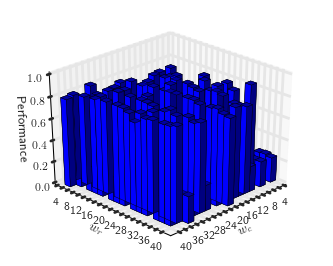
\includegraphics[width=1.0\columnwidth]{img/motivation_1}
\vspace{-1.5em} % Shrink vertical padding
\caption{}
\label{fig:motivation-1}
\end{subfigure}
~%
\begin{subfigure}[h]{.45\columnwidth}
\centering
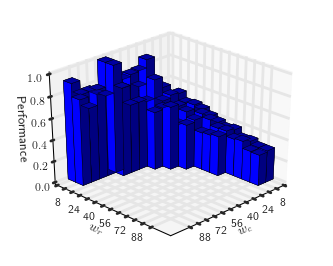
\includegraphics[width=1.0\columnwidth]{img/motivation_2}
\vspace{-1.5em} % Shrink vertical padding
\caption{}
\label{fig:motivation-2}
\end{subfigure}
\caption{%
  The performance of different workgroup sizes for the same stencil
  program on two different devices: (\subref{fig:motivation-1}) Intel
  CPU, (\subref{fig:motivation-2}) NVIDIA GPU. Selecting an
  appropriate workgroup size depends on the execution device.%
}
\label{fig:motivation-arch}
\end{figure}

\begin{figure}
\centering
\begin{subfigure}[h]{.45\columnwidth}
\centering
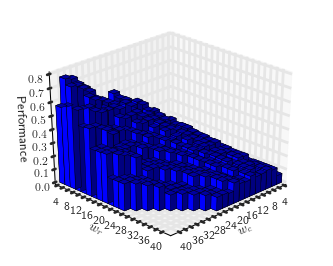
\includegraphics[width=1.0\columnwidth]{img/motivation_3}
\vspace{-1.5em} % Shrink vertical padding
\caption{}
\label{fig:motivation-3}
\end{subfigure}
~%
\begin{subfigure}[h]{.45\columnwidth}
\centering
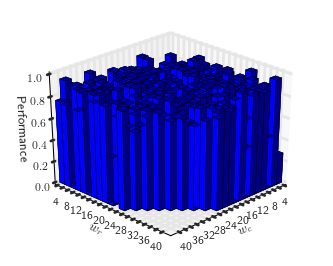
\includegraphics[width=1.0\columnwidth]{img/motivation_4}
\vspace{-1.5em} % Shrink vertical padding
\caption{}
\label{fig:motivation-4}
\end{subfigure}
\caption{%
  The performance of different workgroup sizes for two different
  stencil programs on the same execution device. Selecting an
  appropriate workgroup size depends on the program.%
}
\label{fig:motivation-prog}
\end{figure}


In this section we will briefly examine the performance impact of
selecting workgroup size for the SkelCL Stencil skeleton. A full
explanation of SkelCL and the workgroup size parameter space is given
Section~\ref{sec:omnitune-skelcl}.

SkelCL uses OpenCL to parallelise skeleton operations across many
threads. In OpenCL, multiple threads are grouped into
\emph{workgroups}. The shape and size of these groups is known to have
a big impact on performance. For the SkelCL stencil skeleton, the
selection of workgroup size presents a two dimensional parameter
space, consisting of a number of rows and columns ($w_r \times w_c$).
Measuring and plotting the runtime of stencil programs using different
workgroup sizes allows us to compare the performance of different
workgroup sizes for different combinations of architecture and
program. Figure~\ref{fig:motivation-arch} shows this performance
comparison for a single stencil program on two different devices,
demonstrating that a good choice of workgroup size is device
dependent. The optimization space of the same stencil benchmark on
different devices is radically different: not only does the optimal
workgroup size change between devices, but the performance of
suboptimal workgroup sizes is also dissimilar. The optimization space
of~\ref{fig:motivation-1} has a grid-like structure, with clear
performance advantages of workgroup sizes at multiples of 8 for
$w_c$. A developer specifically targeting this device would learn to
select workgroup sizes following this pattern. This domain specific
knowledge clearly does not transfer to the device shown
in~\ref{fig:motivation-2}.

In Figure~~\ref{fig:motivation-prog}, we compare the performance of
two different stencil programs on the \emph{same} device, showing that
workgroup size choice is also program dependent. In each of these four
examples, the optimal workgroup size changes, as does the relative
performance of suboptimal parameters. The average speedup of the best
over the worst workgroup size is $37.0\times$, and the best average
performance that can be achieved using a single fixed workgroup size
is only 63\% of the maximum.

SkelCL uses a fixed workgroup size by default. Since both the
execution device and the user-provided stencil code are not known
until runtime, selection of workgroup size should be made
dynamically. To the best of our knowledge, there is currently no such
generic system which meets our requirements for lightweight runtime
machine learning autotuning with distributed training sets, and as a
result, a variety of autotuners have been developed ad-hoc and on a
per-case basis.


\section{The OmniTune Framework}\label{sec:autotune}

\begin{figure}
\centering
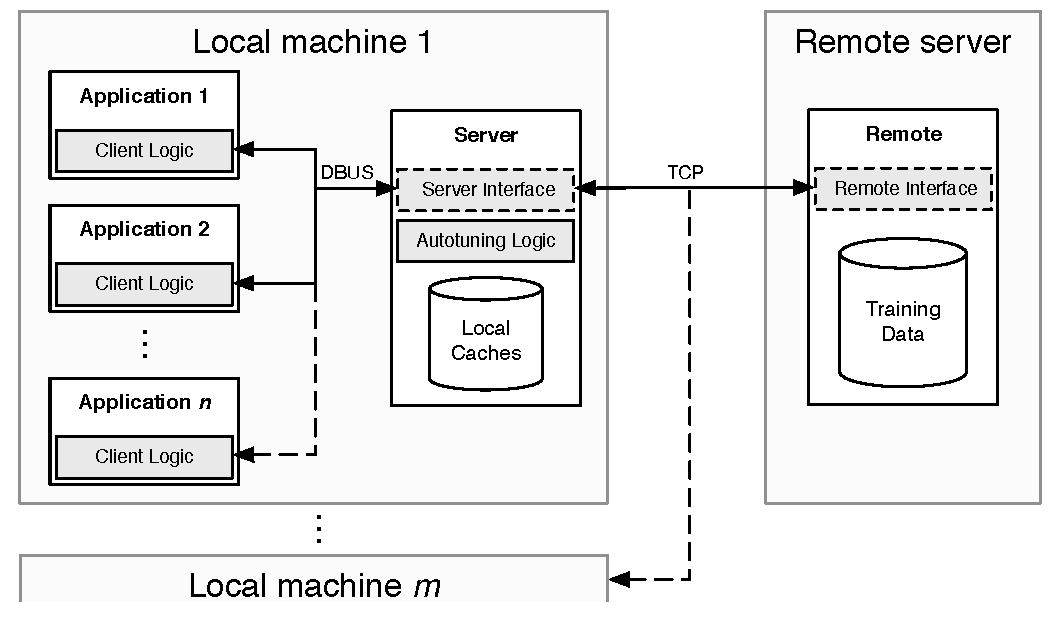
\includegraphics[width=.98\columnwidth]{img/omnitune-system-overview.pdf}
\caption{%
  OmniTune system architecture, showing the separate components and
  the one to many relationship between servers to client applications,
  and remotes to servers.%
  % \vspace{-2em}%
}
\label{fig:omnitune-system-overview}
\end{figure}

OmniTune is a novel framework for extensible, distributed autotuning
of parameter values at runtime using machine learning. It serves as a
generic platform for developing autotuning solutions, aiming to reduce
both the engineering time required to target new optimization
parameters, and the time to deploy on new systems.

It emphasizes collaborative, online learning of optimization spaces. A
client-server architecture with clearly delineated separation of
concerns minimizes the code footprint in client applications, enabling
quick re-purposing for autotuning targets. OmniTune provides a
lightweight interface for communication between each of the
components, and aims to strike a balance between offering a fully
featured environment for quickly implementing autotuning, while
providing enough flexibility to cater to a wide range of use
cases. First, we describe the overall structure of OmniTune and the
rationale for the design, followed by the interfaces and steps
necessary to apply OmniTune.


\subsection{System Architecture}

Common implementations of autotuning in the literature either embed
the autotuning logic within each target application
(e.g.~\cite{Chen2014}), or take a standalone approach in which the
autotuner is a program which must be externally invoked by the user to
tune a target application (e.g.~\cite{Lutz2013}). Embedding the
autotuner within each target application has the advantage of
providing ``always-on'' behavior, but is infeasible for complex
systems in which the cost of building machine learning models must be
added to each program run. The standalone approach separates the
autotuning logic, at the expense of adding one additional step to the
build process. The approach taken in OmniTune aims to combine the
advantages of both techniques by implementing autotuning \emph{as a
  service}, in which a standalone autotuning server performs the heavy
lifting of managing training data and machine learning models, with a
minimal set of lightweight communication logic to be embedded in
target applications.

OmniTune is built around a three tier client-server model, shown in
Figure~\ref{fig:omnitune-system-overview}. The applications which are
to be autotuned are the \emph{clients}. These clients communicate with
a system-wide \emph{server}, which handles autotuning requests. The
server communicates and caches data sourced from a \emph{remote}
server, which maintains a global store of all autotuning data. There
is a many to one relationship between clients, servers, and remotes,
such that a single remote may handle connections to multiple servers,
which in turn may accept connections from multiple clients. This
design has two primary advantages: the first is that it decouples the
autotuning logic from that of the client program, allowing developers
to easily repurpose the autotuning framework to target additional
optimization parameters without a significant development overhead for
the target applications; the second advantage is that this enables
collective tuning, in which training data gathered from a range of
devices can be accessed and added to by any OmniTune server.

The OmniTune framework is implemented as a set of Python classes which
are extended to target specific parameters. The generic implementation
of OmniTune's server and remote components consists of 8987 lines of
Python and MySQL code. No client logic is provided, since that is use
case dependent (See Section~\ref{sec:omnitune-skelcl} for an example
implementation for SkelCL). Inter-process communication between client
programs and the server uses the D-Bus protocol. D-Bus is
cross-platform, and bindings are available for most major programming
languages, allowing flexibility for use with a range of
clients. Communication between servers and remotes uses TCP/IP (we
used an Amazon Web Services database instance for development).


\subsection{Autotuning Behavior}

The goal of machine learning enabled autotuning is to build models
from empirical performance data of past programs to select parameter
values for new \emph{unseen} programs. Instead of an iterative process
of trial and improvement, parameter values are \emph{predicted}, by
building correlations between performance, and \emph{features}
(explanatory variables). The data used to build such models is called
training data. OmniTune supports autotuning using a separate offline
training phase, online training, or a mixture of both. For each
autotuning-capable machine, an OmniTune server acts as an intermediary
between training data and the client application, and hosts the
autotuning logic. On launch, a server requests the latest training
data from the remote, which it uses to build the relevant models for
performing prediction of optimization parameter values. If additional
training data is gathered by the server, this can be uploaded to the
remote.

While the data types of the autotuning interface are
application-specific (e.g. a binary flag or one or more numeric
values), the general pattern is that a client application will request
parameter values from an OmniTune server by sending it a set of
explanatory variables. The server will then use machine learning
models to form a prediction for the optimal parameter values and
return these. Crucially, there is a mechanism provided for the client
to \emph{refuse} parameter values. This functionality is provided for
cases where the predicted parameter values are in some way invalid and
do not lead to a valid program. % TODO: citation

The server contains a library of machine learning tools to perform
parameter prediction, interfacing with the popular datamining software
suite Weka\footnote{\url{http://www.cs.waikato.ac.nz/ml/weka/}} using
its Java Native Interface. The provided tools include classifiers,
regressors, and a selection of meta-learning algorithms.

OmniTune servers may perform additional feature extraction of
explanatory variables supplied by incoming client requests. The reason
for performing feature extraction on the server as opposed to on the
client side is that this allows the results of expensive operations
(for example, analyzing source code of target applications) to be
cached for use across the lifespan of client applications. The
contents of these local caches are periodically and asynchronously
synced with the remote to maintain a global store of lookup tables for
expensive operations.


\subsection{Interfaces}

Key design elements of OmniTune are the interfaces exposed by the
server and remote components. Figure~\ref{fig:omnitune-comms} shows an
example communication pattern between the three components of an
OmniTune system using these interfaces. In the example, a server first
requests training data from the remote. A client application then
performs a training phase in which it requests a set of parameters for
training, evaluates the performance of the parameters, and then
submits a measured value, which the server uses to update the
remote. After training, another client program requests a set of
parameters for performance, refuses them, and makes a new request.

\begin{figure}
\centering
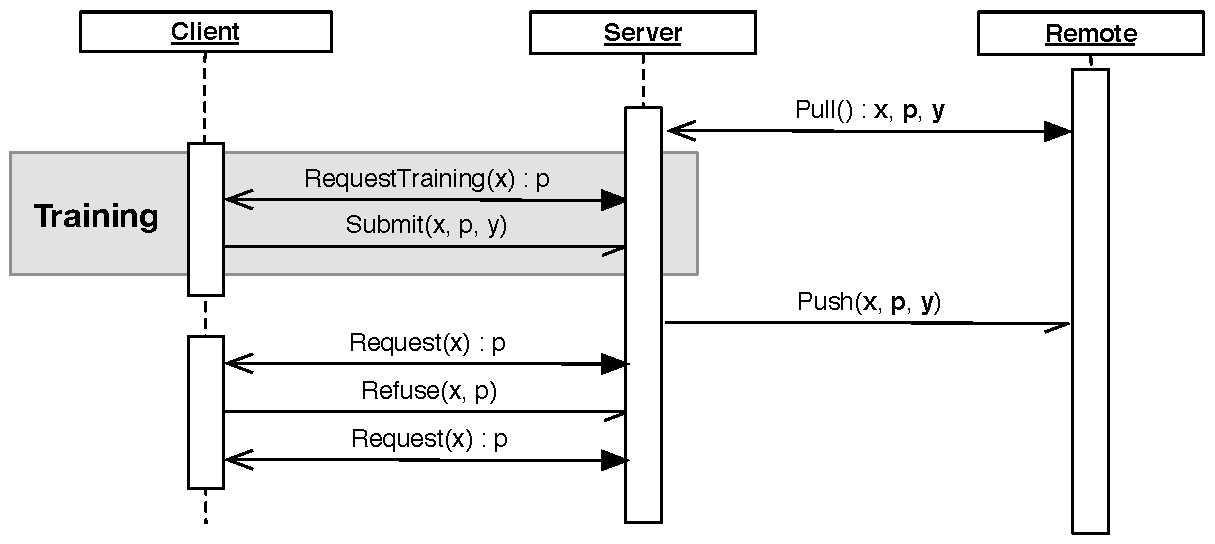
\includegraphics[width=1.0\columnwidth]{img/omnitune-comms}
\caption{%
  An example communication pattern between OmniTune components,
  showing an offline training phase.%
}
\label{fig:omnitune-comms}
\end{figure}

\paragraph{Client-Server} An OmniTune server exposes a public
interface over D-Bus with four operations. Client applications invoke
these methods to request parameter values, submit new training
observations, and refuse suggested parameters:
%
\begin{itemize}
\item \textsc{Request}$(x) \to p$\\*Given explanatory variables $x$,
  request the parameter values $p$ which are expected to provide
  maximum performance.
\item \textsc{RequestTraining}$(x) \to p$\\*Given explanatory
  variables $x$, allow the server to select parameter values $p$ for
  evaluating their fitness.
\item \textsc{Submit}$(x, p, y)$\\*Submit an observed measurement of
  fitness $y$ for parameter values $p$, given explanatory variables
  $x$.
\item \textsc{Refuse}$(x, p)$\\*Refuse parameter values $p$, given a
  set of explanatory variables $x$. Once refused, those parameters are
  blacklisted and will not be returned by any subsequent calls to
  \textsc{Request()} or \textsc{RequestTraining()} for the same
  explanatory variables $x$.
\end{itemize}
%
% This set of operations enables the core functionality of an autotuner,
% while providing flexibility for the client to control how and when
% training data is collected.

\paragraph{Server-Remote} The role of the remote is to provide
bookkeeping of training data for machine learning. Remotes allow
shared access to data from multiple servers using a transactional
communication pattern, supported by two methods:
%
\begin{itemize}
\item \textsc{Push}$(\bf{x}, \bf{p}, \bf{y})$\\*Asynchronously submit
  training data as three lists: explanatory variables $\bf{x}$,
  parameter values $\bf{p}$, and observed outcomes $\bf{y}$.
\item \textsc{Pull}$() \to (\bf{x}, \bf{p}, \bf{y})$\\*Request
  training data as three lists: explanatory variables $\bf{x}$,
  parameter values $\bf{p}$, and observed outcomes $\bf{y}$.
\end{itemize}


\subsection{Extensibility}

To extend OmniTune to target an optimization parameter, a developer
extends the server class to implement response handlers for the four
public interface operations, and then inserts client code into the
target application to call these operations. The implementation of
these response handlers and invoking client code determines the type
of autotuning methods supported. Figure~\ref{fig:omnitune-system-flow}
shows the flow diagram for an example OmniTune implementation. The
call to \textsc{RequestTraining()} is matched with a response call of
\textsc{Submit()}, showing the client recording a training
observation. In the next Section, we will detail the steps required to
apply OmniTune to SkelCL.


\section{Integration of OmniTune with SkelCL}\label{sec:omnitune-skelcl}

\begin{figure}
\centering
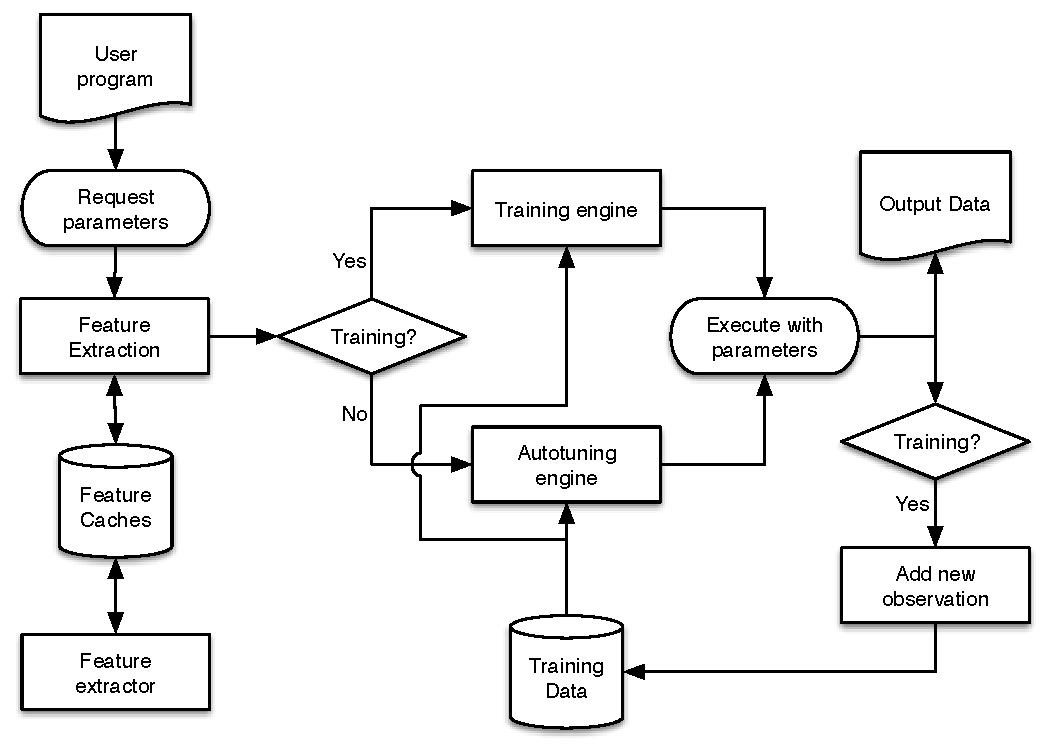
\includegraphics[width=\columnwidth]{img/omnitune-system-flow.pdf}
\caption[Optimization parameter selection with OmniTune]{%
  Predicting parameter values and collecting training data with
  OmniTune.%
}
\label{fig:omnitune-system-flow}
\end{figure}

In this section we demonstrate the practicality of OmniTune by
integrating the framework into an established algorithmic skeleton
library. Introduced in~\cite{Steuwer2011}, SkelCL allows users to
easily harness the power of GPUs and CPUs for data parallel computing,
offering a set of OpenCL implementations of data parallel skeletons in
an object oriented C++ library.

The goal of SkelCL is to enable the transition towards higher-level
programming of GPUs, without requiring users to be intimately
knowledgeable of the concepts unique to OpenCL programming, such as
the memory or execution model. SkelCL has been shown to reduce
programming effort for developing real applications through the use of
robust pattern implementations and automated memory
management. Skeletons are parameterised with user functions which are
compiled into OpenCL kernels for execution on device hardware. SkelCL
supports operations on one or two dimensional arrays of data, with the
Vector and Matrix container types transparently handling lazy
transfers between host and device memory, and supporting partitioning
for multi-GPU execution. SkelCL is freely available and distributed
under dual GPL and academic
licenses\footnote{\url{http://skelcl.uni-muenster.de}}.

\subsection{The Stencil Skeleton}

Stencils are patterns of computation which operate on uniform grids of
data, where the value of each grid element (cell) is updated based on
its current value and the value of one or more neighboring elements,
called the \emph{border region}. Figure~\ref{fig:stencil-img} shows
the use of a stencil to apply a Gaussian blur to an image. SkelCL
provides a 2D stencil skeleton which allows users to provide a
function which updates a cell's value, while SkelCL orchestrates the
parallel execution of this function across all
cells~\cite{Steuwer2014a}.

The border region is described by a \emph{stencil shape}, which
defines an $i \times j$ rectangular region around each cell which is
used to update the cell value. Stencil shapes may be asymmetrical, and
are defined in terms of the number of cells in the border region to
the north, east, south, and west of each cell. Given a function $f$, a
stencil shape $S$, and an $n \times m$ matrix with elements $x_{ij}$:
%
\begin{equation}
\scriptsize
% \begin{split}
\stencil \left( f, S,
\begin{bmatrix}
  x_{11} & \cdots & x_{1m} \\
  \vdots & \ddots & \vdots \\
  x_{n1} & \cdots & x_{nm}
\end{bmatrix} \right)
\to
\begin{bmatrix}
  z_{11} & \cdots & z_{1m} \\
  \vdots & \ddots & \vdots \\
  z_{n1} & \cdots & z_{nm}
\end{bmatrix}
% \end{split}
\end{equation}
%
where:
%
\begin{equation}
\scriptsize
z_{ij} = f \left(
\begin{bmatrix}
  x_{i-S_n,j-S_w} & \cdots & x_{i-S_n,j+S_e} \\
  \vdots & \ddots & \vdots \\
  x_{i+S_s,j-S_w} & \cdots & x_{i+S_s,j+S_e}
\end{bmatrix} \right)
\end{equation}
%
For border region elements outside the bounds of the matrix, values
are substituted from either a predefined padding value, or the value
of the nearest element within the matrix, depending on user
preference.

A popular usage of Stencil codes is for iterative problem solving,
whereby a stencil operation is repeated over a range of discrete time
steps $0 \le t \le t_{max}$, and $t \in \mathbb{N}$. An iterative
stencil operation $g$ accepts a customizing function $f$, a Stencil
shape $S$, and a matrix $M$ with initial values $M_{init}$. The value
of an iterative stencil can be defined recursively as:
%
\begin{equation}
\scriptsize
g(f, S, M, t) =
\begin{cases}
  \stencil \left( f, S, g(f, S, M, t-1) \right),& \text{if } t \geq 1\\
  M_{init}, & \text{otherwise}
\end{cases}
\end{equation}
%
Examples of iterative stencils include cellular automata and partial
differential equation solvers. % Another extension of the stencil
% operation accepts an ordered list of customising functions which are
% applied sequentially for each iteration. This has applications for
% multi-stage stencil operations such as Canny Edge Detection, in
% which four distinct stencil operations are performed as a sequence.

In the implementation of the SkelCL stencil skeleton, each element in
the matrix is mapped to a unique thread (known as a \emph{work item}
in OpenCL) which applies the user-specified function. The work items
are then divided into \emph{workgroups} for execution on the target
hardware. Each work-item reads the value of its corresponding matrix
element and the surrounding elements defined by the border
region. Since the border regions of neighboring elements overlap, the
value of all elements within a workgroup are copied into a
\emph{tile}, allocated as a contiguous region of the fast, but small
local memory. As local memory access times are much faster than that
of global device memory, this greatly reduces the latency of the
border region memory accesses performed by each work item. Changing
the size of workgroups thus affects the amount of local memory
required for each workgroup, and in turn affects the number of
workgroups which may be simultaneously active on the device. While the
user defines the data size and type, the shape of the border region,
and the function being applied to each element, it is the
responsibility of the SkelCL stencil implementation to select an
appropriate workgroup size to use.

\subsection{Optimization Parameters}\label{subsec:op-params}

SkelCL stencil kernels are parameterised by a workgroup size $w$,
which consists of two integer values to denote the number of rows and
columns in a workgroup. The space of optimization parameter values is
subject to hard constraints, and these constraints cannot conveniently
be statically determined. Contributing factors are architectural
limitations, kernel constraints, and parameters which are refused for
other reasons.  Each OpenCL device imposes a maximum workgroup size
which can be statically checked. These are defined by architectural
limitations of how code is mapped to the underlying execution
hardware. Typical values are powers of two, e.g.\ 1024, 4096, 8192. At
runtime, once an OpenCL program has been compiled to a kernel, users
can query the maximum workgroup size supported by that particular
kernel dynamically. This value cannot easily be obtained statically as
there is no mechanism to determine the maximum workgroup size for a
given source code and device without first compiling it, which in
OpenCL does not occur until runtime.

Factors which affect a kernel's maximum workgroup size include the
number of registers required for a kernel, and the available number of
SIMD execution units for each type of instructions in a kernel. In
addition to satisfying the constraints of the device and kernel, not
all points in the workgroup size optimization space are guaranteed to
provide working programs. A \emph{refused parameter} is a workgroup
size which satisfies the kernel and architectural constraints, yet
causes a \texttt{CL\_OUT\_OF\_RESOURCES} error to be thrown when the
kernel is enqueued. Note that in many OpenCL implementations, this
error type acts as a generic placeholder and may not necessarily
indicate that the underlying cause of the error was due to finite
resources constraints. We define a \emph{legal} workgroup size as one
which, for a given \emph{scenario} $s$ (a combination of program,
device, and dataset), satisfies the architectural and kernel
constraints, and is not refused. The subset of all possible workgroup
sizes $W_{legal}(s) \subset W$ that are legal for a given scenario $s$
is then:
%
\begin{equation}
  W_{legal}(s) = \left\{w | w \in W, w < W_{\max}(s) \right\} - W_{refused}(s)
\end{equation}
%
Where $W_{\max}(s)$ can be determined at runtime prior to the kernels
execution, but the set $W_{refused}(s)$ can only be determined
experimentally.


\begin{figure}
\centering
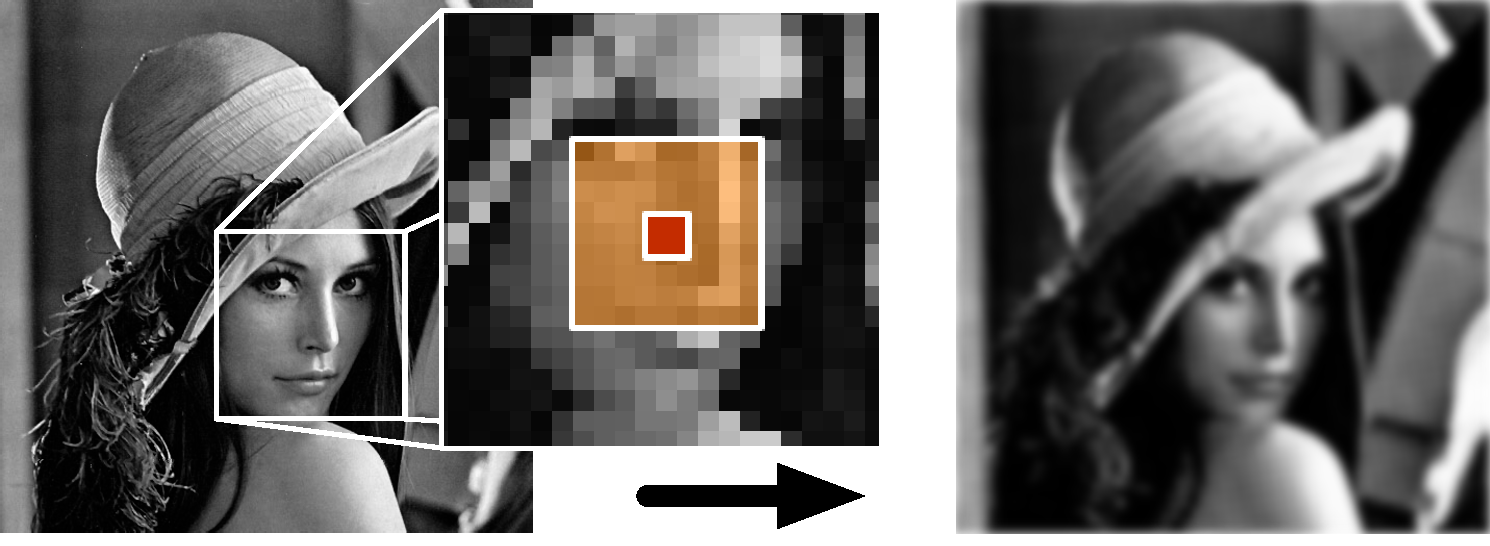
\includegraphics[width=.98\columnwidth]{img/lena-stencil.pdf}
\caption{%
  Application of a Gaussian blur stencil operation to an image, with a
  border region of radius 1. In a Gaussian blur, pixel values are
  interpolated with neighboring pixels, producing a smoothed effect.%
}
\label{fig:stencil-img}
\end{figure}


The \emph{oracle} workgroup size $\Omega(s) \in W_{legal}(s)$ of a
scenario $s$ is the $w$ value which provides the lowest mean
runtime. The relative performance $p(s,w)$ of a particular workgroup
against the maximum available performance for that scenario, within
the range $0 \le p(s,w) \le 1$, is the ratio of the runtime of a
program with workgroup size $w$ over the oracle workgroup size
$\Omega(s)$. For a given workgroup size, the average performance
$\bar{p}(w)$ across a set of scenarios $S$ can be found using the
geometric mean of performance relative to the oracle:
%
\begin{equation}
  \bar{p}(w) =
  \left(
    \prod_{s \in S} p(s, w)
  \right)^{1/|S|}
\end{equation}
%
The \emph{baseline} workgroup size $\bar{w}$ is the value which
provides the best average case performance across a set of
scenarios. Such a baseline value represents the \emph{best} possible
performance which can be achieved using a single, statically chosen
workgroup size. By defining $W_{safe} \in W$ as the intersection of
legal workgroup sizes, the baseline can be found using:
%
\begin{align}
W_{safe} &= \cap \left\{ W_{legal}(s) | s \in S \right\}\\
\bar{w} &= \argmax_{w \in W_{safe}} \bar{p}(w)
\end{align}


\subsection{Machine Learning}

The optimization space presented by the workgroup size of OpenCL
kernels is large, complex, and non-linear. The challenge is to design
a system which, given a set of prior observations of the empirical
performance of stencil codes with different workgroup sizes, predict
workgroup sizes for \emph{unseen} stencils which will maximize the
performance. Successfully applying machine learning requires plentiful
training data, the careful selection of explanatory variables, and
appropriate machine learning methods. For the purpose of this work we
use a \emph{classification} approach, in which a classifier
automatically correlates patterns between explanatory variables and
the workgroup sizes which provide optimal performance. The classifier
used is the popular J48 Decision Tree~\cite{Han2011}, chosen due to
its low classification cost and ability to efficiently handle large
dimensionality training data.

For each scenario, a total of 102 explanatory variables are extracted
to capture information about the device, program, and dataset. Device
variables encode the device type (e.g. CPU or GPU, integrated or
external, connection bus), properties about the host (e.g.\ system
memory, maximum clock frequency), and numerous properties about the
execution device (e.g.\ number of compute units, local memory size,
global caches). Program variables include per-instruction type
densities, the total number of basic blocks, and the total instruction
count. They are extracted using static instruction count passes over
an LLVM IR compiled version of the user stencil
implementation. Compilation to bitcode is a relatively expensive task,
so lookup tables are used to cache repeated uses of the same stencil
codes, identified by a checksum of the source code. Dataset variables
include the data type and dimensions of the SkelCL container type.

To collect training data, we run multiple iterations of a stencil
program to enumerate the workgroup size optimization space, and use
the OpenCL's Profiling API to record stencil kernel execution times in
the client application, which are then submitted to the OmniTune
server. The \textsc{RequestTraining}$(x)$ server interface returns a
workgroup size with a randomly selected even number of rows and
columns that obeys the maximum size constraints.

A parameterised template substitution engine is used to generate
synthetic stencil applications for gathering performance
data. Stencils templates are parameterised with a border region size
and \emph{complexity}, a simple metric to broadly dictate the number
of operations in a given stencil code.

Once the performance of different workgroup sizes for a scenario is
assessed, the set of explanatory variables describing the scenario is
paired with the oracle workgroup size. This process is repeated for
multiple scenarios to create training data. A classifier learns from
this training data to make predictions for new sets of explanatory
variables, by predicting a workgroup size from the set of oracle
workgroup sizes of the training data.

This approach presents the problem that after training, there is no
guarantee that the set of workgroup sizes which may be predicted is
within the set of legal workgroup sizes for future scenarios. This may
result in a classifier predicting a workgroup size which is not legal
for a scenario, $w \not\in W_{legal}(s)$, either because it exceeds
$W_{\max}(s)$, or because the parameter is refused. If this occurs, a
\emph{nearest neighbor} approach is used to select the workgroup size
$w$ which is expected to be legal and has the lowest Euclidian
distance to the predicted value $c$. This is achieved by comparing row
($r$) and column ($c$) indices:
%
\begin{equation}
  w = \underset{w \in W_{legal(s)}}{\argmin} \sqrt{\left(c_r - w_r\right)^2 + \left(c_c - w_c\right)^2}
\end{equation}
%
This process of selecting alternative parameters will iterate until a
legal parameter is found.

\subsection{Implementation}

\begin{figure}
\begin{subfigure}[h]{.32\columnwidth}
\centering
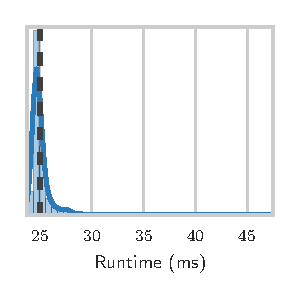
\includegraphics[width=\textwidth]{img/runtimes_histogram_1}
\vspace{-1.5em} % Shrink vertical padding
\caption{}
\label{fig:runtimes-histogram-1}
\end{subfigure}
~%
\begin{subfigure}[h]{.32\columnwidth}
\centering
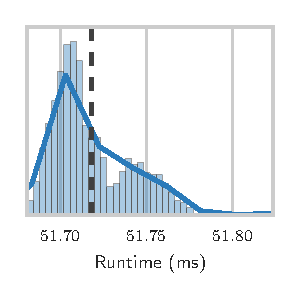
\includegraphics[width=\textwidth]{img/runtimes_histogram_2}
\vspace{-1.5em} % Shrink vertical padding
\caption{}
\label{fig:runtimes-histogram-2}
\end{subfigure}
~%
\begin{subfigure}[h]{.32\columnwidth}
\centering
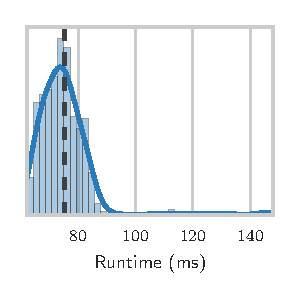
\includegraphics[width=\textwidth]{img/runtimes_histogram_3}
\vspace{-1.5em} % Shrink vertical padding
\caption{}
\label{fig:runtimes-histogram-3}
\end{subfigure}
\\
\begin{subfigure}[h]{.32\columnwidth}
\centering
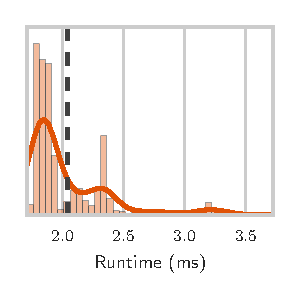
\includegraphics[width=\textwidth]{img/runtimes_histogram_4}
\vspace{-1.5em} % Shrink vertical padding
\caption{}
\label{fig:runtimes-histogram-4}
\end{subfigure}
~%
\begin{subfigure}[h]{.32\columnwidth}
\centering
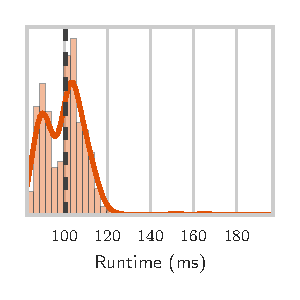
\includegraphics[width=\textwidth]{img/runtimes_histogram_5}
\vspace{-1.5em} % Shrink vertical padding
\caption{}
\label{fig:runtimes-histogram-5}
\end{subfigure}
~%
\begin{subfigure}[h]{.32\columnwidth}
\centering
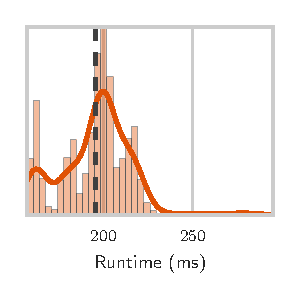
\includegraphics[width=\textwidth]{img/runtimes_histogram_6}
\vspace{-1.5em} % Shrink vertical padding
\caption{}
\label{fig:runtimes-histogram-6}
\end{subfigure}
\\
\begin{subfigure}[h]{.32\columnwidth}
\centering
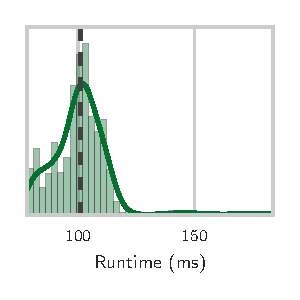
\includegraphics[width=\textwidth]{img/runtimes_histogram_7}
\vspace{-1.5em} % Shrink vertical padding
\caption{}
\label{fig:runtimes-histogram-7}
\end{subfigure}
~%
\begin{subfigure}[h]{.32\columnwidth}
\centering
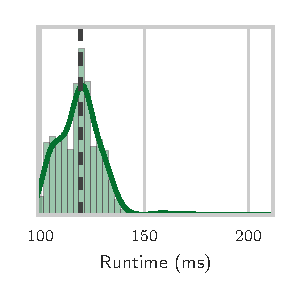
\includegraphics[width=\textwidth]{img/runtimes_histogram_8}
\vspace{-1.5em} % Shrink vertical padding
\caption{}
\label{fig:runtimes-histogram-8}
\end{subfigure}
~%
\begin{subfigure}[h]{.32\columnwidth}
\centering
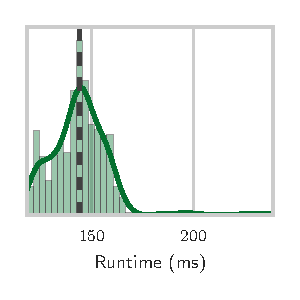
\includegraphics[width=\textwidth]{img/runtimes_histogram_9}
\vspace{-1.5em} % Shrink vertical padding
\caption{}
\label{fig:runtimes-histogram-9}
\end{subfigure}
\caption[Distribution of stencil code runtimes]{%
  Distribution of runtime samples for test cases from three
  devices. Each plot contains a 35-bin histogram of 1000 samples, and
  a fitted kernel density estimate with bandwidth 0.3. The sample mean
  is shown as a vertical dashed line. The top row are from the Intel
  i5-4570, the second row from the Nvidia GTX 590, and the third row
  from the AMD Tahiti 7970. In some of the plots, the distribution of
  runtimes is bi- or multi-modal, and skewed to the lower end of the
  runtimes range.%
}
\label{fig:runtime-histograms}
\end{figure}

The OmniTune framework consists of 8987 lines of Python and MySQL
code. A further 976 lines are required for the SkelCL frontend to
implement the server response handlers and database backend. By
design, the client-server model minimizes the impact of number of
modifications that are required to enable autotuning in client
applications. The only modification required to SkelCL is to replace
the hardcoded values for workgroup size with a subroutine to request a
workgroup size from the OmniTune server over a D-Bus connection. To
use the system, a user must download a copy of SkelCL modified with
the OmniTune functionality, and start a local OmniTune server
instance. A configuration file is used to determine the domain address
and authentication details of the remote server. On first launch, the
OmniTune server will fetch the latest training data from the remote.


\section{Experimental Setup}

This section describes an exhaustive enumeration of the workgroup size
optimization space for 429 combinations of architecture, program, and
dataset. It contains the methodology used to collect empirical
performance data on which to base performance comparisons of different
workgroup sizes, and the steps necessary to obtain repeatable results.

A full enumeration of the workgroup size optimization spaces was
performed across synthetically generated benchmarks and four reference
stencil benchmarks: Canny Edge Detection, Conway's Game of Life, Heat
Equation, and Gaussian Blur. Performance data was collected from 7
experimental platforms, comprising 4 GPU devices: AMD Tahiti 7970,
Nvidia GTX 590, Nvidia GTX 690, Nvidia GTX TITAN; and 3 CPU devices:
Intel i5-2430M, Intel i5-4570, i7-3820. Each platform was unloaded,
frequency governors disabled, and benchmark processes set to the
highest priority available to the task scheduler. Datasets and
programs were stored in an in-memory file system. For each program,
dataset sizes of size $512\times512$, $1024\times1024$,
$2048\times2048$, and $4096\times4096$ were used. A minimum of 30
samples were recorded for each scenario and workgroup size.

Program behavior is validated by comparing program output against a
gold standard output collected by executing each of the real-world
benchmarks programs using the baseline workgroup size. The output of
real-world benchmarks with other workgroup sizes is compared to this
gold standard output to test for correct program execution.


\section{Evaluation}\label{sec:evaluation}

This section evaluates the performance of OmniTune when tasked with
selecting workgroup sizes for SkelCL stencil codes. The experimental
results consist of measured runtimes for a set of \emph{test cases},
where each test case $\tau_i$ consists of a scenario, workgroup size
pair $\tau_i = (s_i,w_i)$, and is associated with a \emph{sample} of
observed runtimes from multiple runs of the program. A total of
269,813 test cases have been evaluated with an average sample size of
83 (min 33, total 16,917,118). This represents an exhaustive
enumeration of the workgroup size optimization space for 429
scenarios, with an average of 629 (max 7,260) unique workgroup sizes
for each scenario.


\subsection{Runtime Noise}

\begin{figure}
\centering
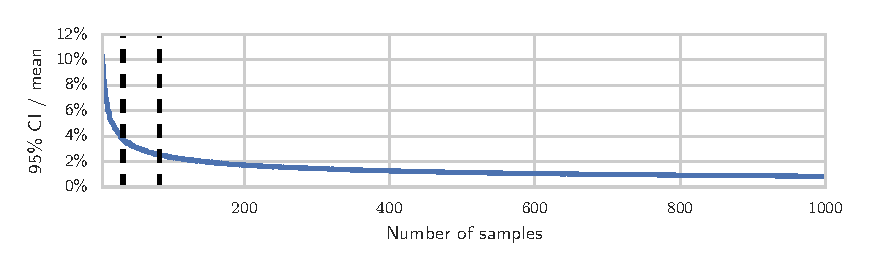
\includegraphics[width=\columnwidth]{img/ci_trend}
\caption[Confidence interval size vs.\ sample count]{%
  Ratio of 95\% confidence interval to mean as a function of sample
  size. Two dashed lines indicate the confidence intervals at the
  minimum (3.7\%) and mean (2.5\%) sample size found in the
  experimental dataset.%
}
\label{fig:ci-trends}
\end{figure}

First we examine the noise present in program runtime
measurements. The complex interaction between processes competing for
the finite resources of a system introduces many sources for such
noise. Figure~\ref{fig:runtime-histograms} plots the distributions of
1000 runtimes recorded for 9 SkelCL stencil kernels, (a)--(i). The
plots show that the distribution of runtimes is not Gaussian; rather,
it is sometimes multimodal, and generally skewed to the lower end of
the runtime range, with a long ``tail'' to the right. This fits our
intuition that programs have a hard \emph{minimum} runtime enforced by
the time taken to execute the instructions of a program, and that
noise introduced to the system extends this runtime. For example,
preempting an OpenCL process on a CPU so that another process may run
may cause the very long tail visible in
Figure~\ref{fig:runtimes-histogram-1}.

It is important to ensure a sufficiently large sample size when
performing optimisations based on empirical performance data. A
recommendation of $\ge 30$ samples is common in the benchmarking
literature~\cite{Georges2007}. Our experimental results support this
recommendation: Figure~\ref{fig:ci-trends} plots the ratio of 95\%
confidence interval to the sample mean for different sample sizes,
showing a 50\% reduction in confidence interval size when increasing
the sample size from 10 to 30. In this experimental dataset, the ratio
of confidence interval to mean at the smallest sample size (33) is
3.7\%, and 2.5\% at the mean sample size (83).


\subsection{OpenCL Workgroup Size Optimization Space}

\begin{figure}
\centering
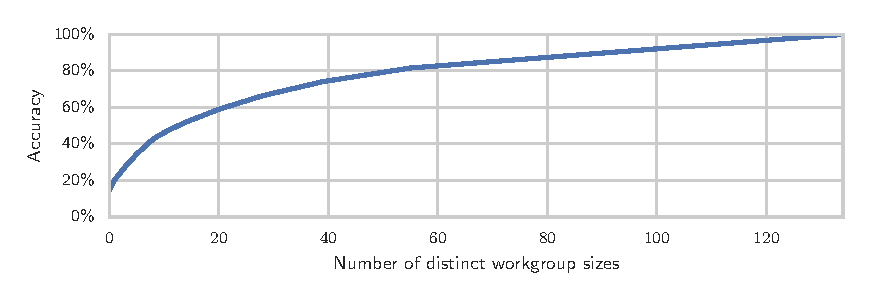
\includegraphics[width=\columnwidth]{img/num_params_oracle.pdf}
\caption{%
  Accuracy compared to the oracle as a function of the number of
  unique workgroup sizes. The greatest accuracy that can be achieved
  using a single statically chosen workgroup size is 15\%. Achieving
  50\% oracle accuracy requires a minimum of 14 distinct workgroup
  sizes.%
}
\label{fig:oracle-accuracy}
\end{figure}

We can calculate an upper bound for the performance impact of the
workgroup size parameter by comparing the average runtimes of the
\emph{best} and \emph{worst} workgroup size for a single
scenario. Applying this to all scenarios, we find the average speedup
upper bound to be $15.14\times$ (min $1.03\times$, max
$207.72\times$). This demonstrates the importance of tuning stencil
workgroup sizes --- if chosen incorrectly, the runtime of stencil
programs can be extended by up to $207.72\times$. Note that for 5 of
the scenarios, the speedup of the best over worst workgroup sizes is
less than $5\%$. For these scenarios, there is little benefit to
autotuning; however, this represents only 1.1\% of the tested
scenarios. For 50\% of the scenarios, the speedup of the best over
worst workgroup sizes is greater than $6.19\times$.

For the purposes of evaluating autotuning, we use three
\emph{baselines} to compare program runtimes against. The relative
performance of a workgroup size for a particular scenario is compared
against runtimes for one of three parameters:
%
\begin{itemize}
\item \emph{Oracle} --- The \emph{oracle} workgroup size is the
  workgroup size which provided the lowest mean runtime for a given
  scenario. Speedup relative to the oracle is in the range
  $0 \le x \le 1$, so this can be referred to as \emph{performance}.
\item \emph{Baseline} --- The \emph{baseline} parameter is the
  workgroup size which provides the best overall performance while
  being legal for all scenarios. For our experimental data, we find
  this value to be $w_{(4 \times 4)}$.
\item \emph{Human expert} --- In the original implementation of the
  SkelCL stencil skeleton~\cite{Steuwer2014a},
  \citeauthor{Steuwer2014a} selected a workgroup size of
  $w_{(32 \times 4)}$, based on an evaluation of 4 stencil programs on
  a Tesla S1070 system.
\end{itemize}
%
Across the 429 scenarios tested, there are 135 unique \emph{oracle}
workgroup sizes. This demonstrates the difficulty in attempting to
statically tune for \emph{optimal} parameter values, since 31.5\% of
scenarios have different oracle workgroup
sizes. Figure~\ref{fig:oracle-accuracy} shows that a minimum of 14
distinct workgroup sizes are needed to achieve just 50\% of the oracle
accuracy, although it is important to make the distinction that oracle
\emph{accuracy} and \emph{performance} are not equivalent.

We find that the \emph{human expert} selected workgroup size is
invalid for 2.6\% of scenarios, as it is refused by 11 test cases. By
device, these are: 3 on the GTX 690, 6 on the i5-2430M, and 2 on the
i5-4570. For the purpose of comparing performance against human
experts, we will ignore these test cases, but it demonstrates the
utility of autotuning not just for maximizing performance, but
ensuring program reliability. For the scenarios where the human expert
workgroup size \emph{is} legal, it achieves an impressive geometric
mean of 79.2\% of the oracle performance. The average speedup of
oracle workgroup sizes over the workgroup size selected by a human
expert is $1.37\times$ (min $1.0\times$, max $5.17\times$).

The utility of the \emph{baseline} workgroup size is that it
represents the best performance that can be achieved through static
tuning. The baseline workgroup size achieves only 24\% of the maximum
performance. Figures~\ref{fig:performance-wgsizes}
and~\ref{fig:performances} show box plots for the performance of all
workgroup sizes using different groupings: ratio of maximum workgroup
size, kernel, device, and dataset. The plots show the median
performance, interquartile range, and outliers. What is evident is
both the large range of workgroup size performances (i.e. the high
performance upper bounds), and the lack of obvious correlations
between any of the groupings and performance.


\begin{figure}
  \begin{subfigure}[h]{\columnwidth}
    \centering
    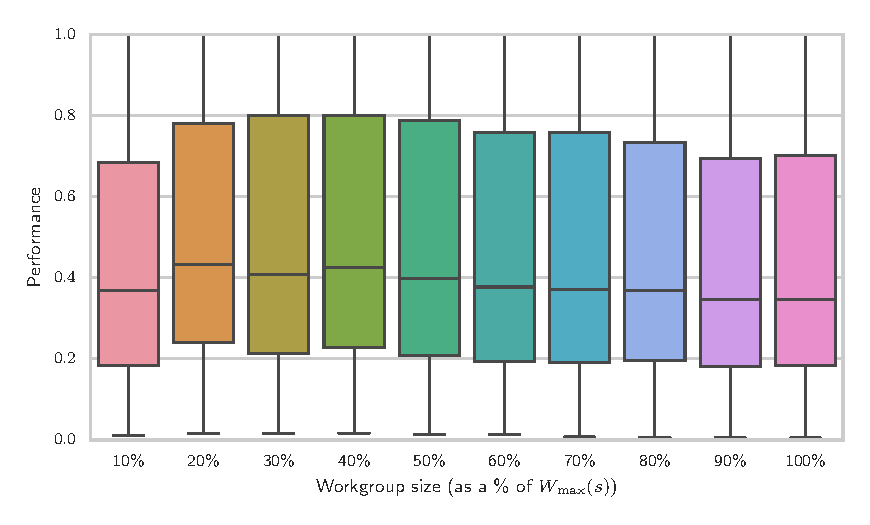
\includegraphics[width=\columnwidth]{img/performance_max_wgsize}
    \vspace{-1.5em} % Shrink vertical padding
    \caption{}
    \label{fig:performance-max-wgsize}
  \end{subfigure}
  \\
  \begin{subfigure}[h]{.48\columnwidth}
    \centering
    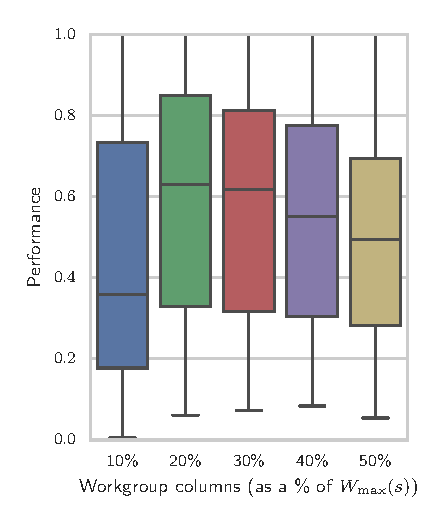
\includegraphics[width=\columnwidth]{img/performance_max_c}
    \vspace{-1.5em} % Shrink vertical padding
    \caption{}
    \label{fig:performance-wg-c}
  \end{subfigure}
  ~%
  \begin{subfigure}[h]{.48\columnwidth}
    \centering
    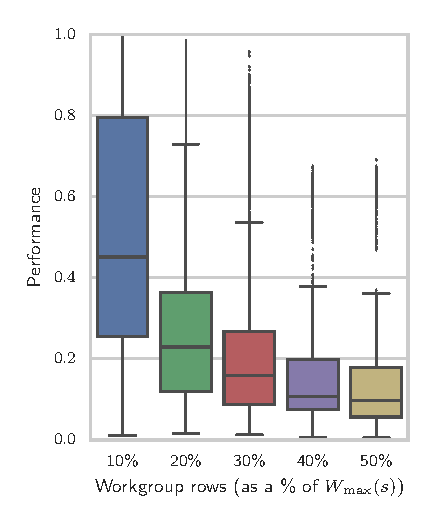
\includegraphics[width=\columnwidth]{img/performance_max_r}
    \vspace{-1.5em} % Shrink vertical padding
    \caption{}
    \label{fig:performance-wg-r}
  \end{subfigure}
  \caption{%
    Comparing performance of workgroup sizes relative to the oracle as
    a function of: (\subref{fig:performance-max-wgsize})~maximum legal
    size, (\subref{fig:performance-wg-c})~number of columns, and
    (\subref{fig:performance-wg-r})~number of rows. Each workgroup
    size is normalized to the maximum allowed for that scenario,
    $W_{\max}(s)$. There is no clear correlation between workgroup
    size and performance.%
  }
  \label{fig:performance-wgsizes}
\end{figure}

\begin{figure}
  \begin{subfigure}[h]{\columnwidth}
    \centering
    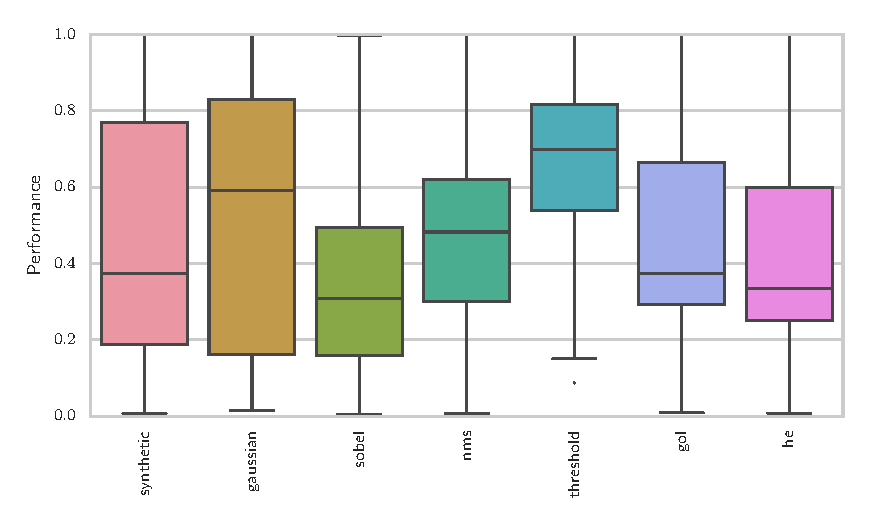
\includegraphics[width=\columnwidth]{img/performance_kernels.pdf}
    \vspace{-1.5em} % Shrink vertical padding
    \caption{}
    \label{fig:performance-kernels}
  \end{subfigure}
  \\
  \begin{subfigure}[h]{.48\columnwidth}
    \centering
    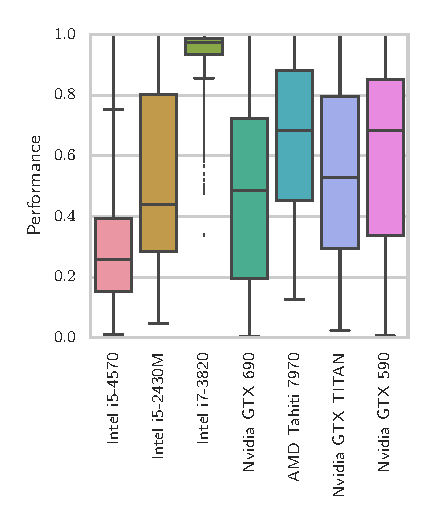
\includegraphics[width=\columnwidth]{img/performance_devices.pdf}
    \vspace{-1.5em} % Shrink vertical padding
    \caption{}
    \label{fig:performance-devices}
  \end{subfigure}
  ~%
  \begin{subfigure}[h]{.48\columnwidth}
    \centering
    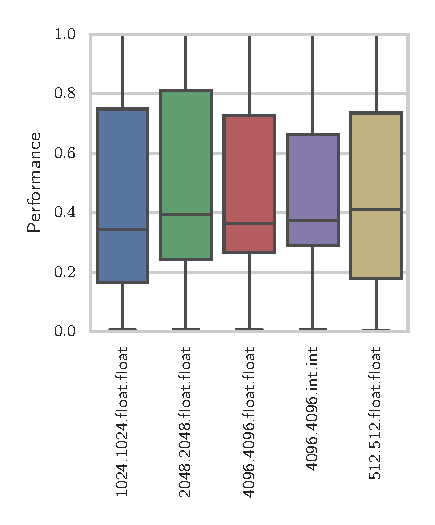
\includegraphics[width=\columnwidth]{img/performance_datasets.pdf}
    \vspace{-1.5em} % Shrink vertical padding
    \caption{}
    \label{fig:performance-datasets}
  \end{subfigure}
  \caption{%
    Performance relative to the oracle of workgroup sizes across all
    test cases, grouped by:
    (\subref{fig:performance-kernels})~kernels,
    (\subref{fig:performance-devices})~devices, and
    (\subref{fig:performance-datasets})~datasets. The performance
    impact is not consistent across kernels, devices, or datasets. The
    Intel i7-3820 has the lowest performance gains from tuning
    workgroup size.%
  }
  \label{fig:performances}
\end{figure}

\subsection{Autotuning Workgroup Sizes}

To evaluate the performance of machine learning-enabled autotuning of
SkelCL stencils, we partition the experimental data into
\emph{training} and \emph{test} sets. The training set is used to
build the machine learning model. The predicted workgroup size for
each entry in the test set is then used to evaluate the autotuning
performance. We use 5 different approaches to partitioning the test
and training data, which each test different aspects of the
system. The first is a $k$-fold cross validation, a standard machine
learning model validation technique in which the set of all data is
shuffled and then divided into $k$ equally sized validation sets. Each
validation set is used to test a model trained on the remaining
data~\cite{Han2011}. In our evaluation we use a value of $k=10$. The
second technique is to partition the data such that it consists of
data gathered from synthetic benchmarks, and use data collected from
real-world benchmarks to test. This tests the utility of training
using synthetically generated benchmarks. The third, forth, and fifth
approaches involve creating leave-one-out training sets for all data
grouped by device, kernel, and dataset, respectively. This tests the
ability to successfully apply prior knowledge about other devices,
kernels, and datasets, to new unseen cases. For example, of the $n$
devices used to collect performance data, the model is trained on data
from $n-1$ devices, and tested against data from the
$n^{th}$. Table~\ref{tab:class} summarizes the results of evaluating
the autotuner using each of the different validation techniques.

The autotuner achieves good performance, with average speedups over
the baseline across all validation sets range between $4.79\times$ and
$5.65\times$. Importantly, the performance when validating across
devices, kernels, and datasets, is comparable to the 10-fold
validation. This demonstrates that the autotuner is capable of
learning \emph{across} these targets. So if the autotuner is deployed
to a system for which it has no prior knowledge, it does not suffer a
significant drop in performance. The same is true for an unseen
kernel, or dataset type. This, combined with the distributed datasets
provided by the OmniTune framework, demonstrates the utility of
autotuning at the skeletal level, allowing machine learning to
successfully learn predictions across unseen programs, kernels, and
datasets.

Classification using decision trees is a lightweight process (they can
be implemented using a chain of \texttt{if}/\texttt{else} statements).
The measured overhead of autotuning is 2.5ms, of which only 0.3ms is
required for classification using Weka, although an optimized decision
tree implementation could reduce this further. The remaining 2.2ms is
required for feature extraction and the inter-process round trip
between the OmniTune server and client.


\begin{table}
\scriptsize
\centering
\begin{tabular}{llL{1.5cm}L{1.6cm}}
\toprule
Training Dataset & Performance & Speedup over Baseline & Speedup over Human Expert \\
\midrule
10-fold & 92\% & $5.65\times$ &       $1.26\times$ \\
Synthetic & 92\% & $4.79\times$ &       $1.13\times$ \\
$n-1$ Device & 85\% & $5.23\times$ &       $1.17\times$ \\
$n-1$ Kernel & 89\% & $5.43\times$ &       $1.21\times$ \\
$n-1$ Dataset & 91\% & $5.63\times$ &       $1.25\times$ \\
 \textbf{Average} &  \textbf{90\%} &  $\bm{5.45\times}$ &  $\bm{1.22\times}$ \\
\bottomrule
\end{tabular}
\caption{%
  Performance results using a J48 Decision Tree across different
  validation sets. Note that the human expert selected workgroup size
  is invalid for 2.6\% of test cases, which we excluded for the
  purpose of performance comparisons against human expert.%
}
\label{tab:class}
\end{table}

\subsection{OmniTune Extensibility}

The client-server architecture OmniTune neatly separates the
autotuning logic from the target application. This makes adjusting the
autotuning methodology a simple process. To demonstrate this, we
changed the machine learning algorithm from a J48 decision tree to a
Naive Bayes classifier, and duplicated the evaluation. This required
only a single line of source code in the OmniTune server extension to
be changed. Figure~\ref{fig:class-hmaps} visualizes the differences in
autotuning predictions when changing between these two
classifiers. While the average performances of the two classifiers is
comparable, the distribution of predictions is not. For example, the
Naive Bayes classifier predicted the human expert selected workgroup
size of $w_{(32 \times 4)}$ more frequently than it was optimal, while
the decision tree predicted it less frequently. Selection of machine
learning algorithms has a large impact on the effectiveness of
autotuning, and the OmniTune client-server design allows for low cost
experimenting with different approaches. In future work we will
investigate meta-tuning techniques for selecting autotuning
algorithms.


\begin{figure}
\centering
\begin{subfigure}[t]{0.48\columnwidth}
\centering
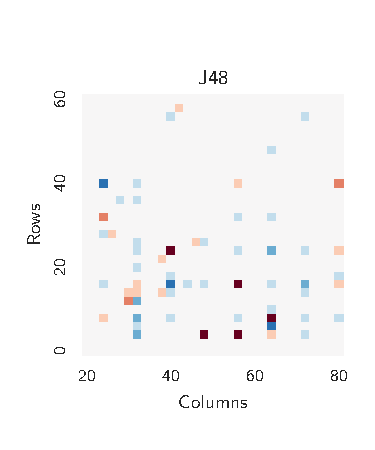
\includegraphics[width=\columnwidth]{img/heatmap_1}
\vspace{-1.5em} % Shrink vertical padding
\caption{}
\label{fig:class-hmaps-1}
\end{subfigure}
\begin{subfigure}[t]{0.48\columnwidth}
\centering
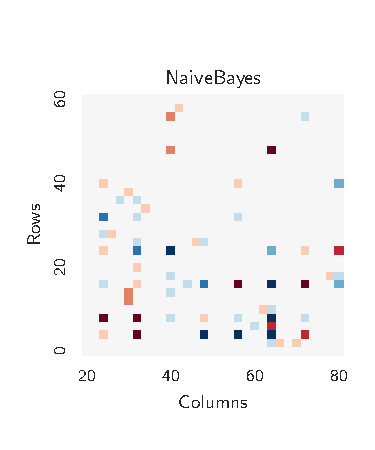
\includegraphics[width=\columnwidth]{img/heatmap_2}
\vspace{-1.5em} % Shrink vertical padding
\caption{}
\label{fig:class-hmaps-2}
\end{subfigure}
% \\
% \begin{subfigure}[t]{0.48\columnwidth}
% \centering
% 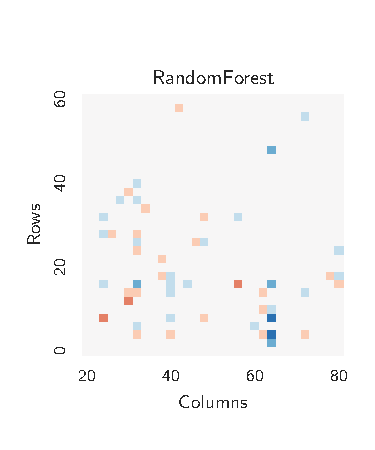
\includegraphics[width=\columnwidth]{img/heatmap_3}
% \vspace{-1.5em} % Shrink vertical padding
% \caption{}
% \label{fig:class-hmaps-3}
% \end{subfigure}
% \begin{subfigure}[t]{0.48\columnwidth}
% \centering
% 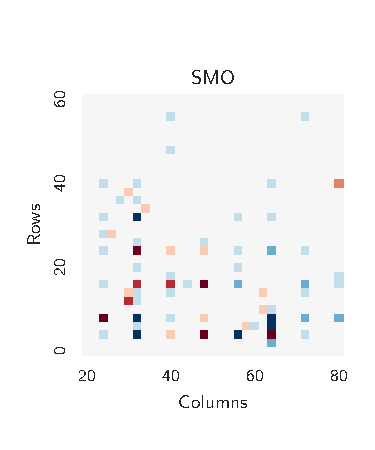
\includegraphics[width=\columnwidth]{img/heatmap_5}
% \vspace{-1.5em} % Shrink vertical padding
% \caption{}
% \label{fig:class-hmaps-4}
% \end{subfigure}
\caption{%
  Heatmaps of autotuner predictions for a subset of the optimization
  space using two different classifiers. The shading in each cells
  indicates if it is predicted less frequently (blue), ore more
  frequently (red) than it is optimal. Color gradients are normalized
  across plots.%
}
\label{fig:class-hmaps}
\end{figure}


\subsection{Summary}

In this section we have explored the performance impact of the
workgroup size optimization space, and the effectiveness of autotuning
using OmniTune to exploit this. By comparing the relative performance
of an average of 629 workgroup sizes for each of 429 scenarios, the
following conclusions can be drawn:

%
\begin{itemize}
\item The performance gap between the best and workgroup sizes for a
  particular combination of hardware, software, and dataset is up to
  $207.72\times$.
\item Not all workgroup sizes are legal, and the space of legal
  workgroup sizes cannot statically be determined. Adaptive tuning is
  required to ensure reliable performance.
\item Statically tuning workgroup size fails to extract the potential
  performance across a range of programs, architectures, and
  datasets. The best statically chosen workgroup size achieves only
  26\% of the optimal performance.
\item Workgroup size prediction using a decision tree achieves an
  average 90\% of the optimal performance.
\item Auotuning provides performance portability across programs,
  devices, and datasets. The performance of predicted workgroup sizes
  for unseen devices is within 8\% of the performance for known
  devices.
\end{itemize}


\section{Related Work}\label{sec:related}

Early work in autotuning applied iterative search techniques to the
space of compiler optimisations~\cite{Bodin1998,Kisuki}. Since then,
machine learning techniques have been successfully employed to reduce
the cost of iterative
compilation~\cite{Agakov,Stephenson2003,Fursin2011}. However,
optimizing GPGPU programs presents different challenges to that of
traditional CPU programming. \citeauthor{Ryoo2008a} demonstrated
speedups of up to $432\times$ for matrix multiplication in CUDA
through the appropriate use of zero-overhead thread scheduling, memory
bandwidth, and thread grouping. The importance of proper exploitation
of local shared memory and synchronization costs is explored
in~\cite{Lee2010}. In~\cite{Chen2014}, data locality optimisations are
automated using a description of the hardware and a
memory-placement-agnostic compiler. \citeauthor{Magni2014} use a
machine learning model to predict optimal thread coarsening factors of
OpenCL kernels in~\cite{Magni2014}, demonstrating speedups between
$1.11\times$ and $1.33\times$.

Auotuning transformations for stencil codes are explored
in~\cite{Kamil2010} using an IR to represent stencils and a CUDA code
generator at the backend. However, they do not optimize for the GPU
memory hierarchy, using only global memory. In~\cite{Lutz2013},
\citeauthor{Lutz2013} demonstrate that optimal swapping strategy for
multi-GPU stencils depends on the size of the grid, the number of
partitions, and the connection mechanism (e.g.\ PCI express).

OpenTuner is a general purpose toolkit for autotuning which uses
ensemble search techniques to reduce the cost of exploring an
optimization space, rather than the machine learning approach taken in
this work~\cite{Ansel2013}. Since OpenTuner does not \emph{learn}
optimization spaces as OmniTune does, performance data is not shared
across devices. This means that the search for performant parameter
values must be performed by each new device to be autotuned. Our
approach combines machine learning with distributed training sets so
that new users automatically benefit from the collective tuning
experience of other users, which reduces the time to deployment.

A ``big data'' driven approach to autotuning is presented
in~\cite{Fursin2014}. The authors propose the use of ``Collective
optimization'' to leverage training experience across devices, by
sharing performance data, datasets and additional metadata about
experimental setups. In addition to the mechanism for sharing training
datasets, our system provides the capabilities of performing
autotuning at runtime using a lightweight inter-process communication
interface. Additionally, Collective Mind uses a NoSQL JSON format for
storing datasets. The relational schema used in OmniTune offers
greater scaling performance and lower storage overhead as the amount
of performance data grows. The authors do not provide an empirical
evaluation of their technique.


\section{Conclusions}\label{sec:conclusions}

As the trend towards increasingly programmable heterogeneous
architectures continues, the need for high level, accessible
abstractions to manage such parallelism will continue to
grow. Autotuning proves to be a valuable aid for achieving these
goals, provided that the burden of development and collecting
performance data is lifted from the user. The system presented in this
paper aims to solve this issue by providing a generic interface for
implementing machine learning-enabled autotuning. OmniTune is a novel
framework for autotuning which has the benefits of a fast, ``always-on''
interface for client applications, while being able to synchronize
data with global repositories of knowledge which are built up across
devices. To demonstrate the utility of this framework, we implemented
a frontend for predicting the workgroup size of OpenCL kernels for
SkelCL stencil codes. This optimization space is complex, non linear,
and critical for the performance of stencil kernels. Selecting the
correct workgroup size is difficult --- requiring a knowledge of the
kernel, dataset, and underlying architecture. The implemented
autotuner achieves 92 \% of the maximum performance, and is provides
performance portability, even achieving an average of 85\% of the
maximum performance when deployed on a device for which it has no
prior training data. In future work we will explore methods for
collaborative exploration of optimization spaces in parallel across
multiple cooperating devices.

\acks

This work was supported by the UK Engineering and Physical Sciences
Research Council under grants EP/L01503X/1 for the University of
Edinburgh School of Informatics Centre for Doctoral Training in
Pervasive Parallelism
(\url{http://pervasiveparallelism.inf.ed.ac.uk/}), EP/H044752/1
(ALEA), and EP/M015793/1 (DIVIDEND).

\label{bibliography}
\printbibliography


\end{document}
